% \documentclass[aip,jcp,preprint,unsortedaddress,a4paper,onecolum]{revtex4-1}
\documentclass[aip,jcp,a4paper,reprint,onecolumn]{revtex4-1}
% \documentclass[aps,pre,twocolumn]{revtex4-1}
% \documentclass[aps,jcp,groupedaddress,twocolumn,unsortedaddress]{revtex4}

\usepackage[fleqn]{amsmath}
\usepackage{amssymb}
\usepackage[dvips]{graphicx}
\usepackage{color}
\usepackage{tabularx}
\usepackage{algorithm}
\usepackage{algorithmic}

\makeatletter
\makeatother

\newcommand{\recheck}[1]{{\color{red} #1}}
\newcommand{\redc}[1]{{\color{red} #1}}
\newcommand{\bluec}[1]{{\color{blue} #1}}
\newcommand{\vect}[1]{\textbf{\textit{#1}}}
\newcommand{\dd}[1]{\textsf{#1}}

\newcommand{\AT}{{\textrm{{AT}}}}
\newcommand{\EX}{{\textrm{EX}}}
\newcommand{\CG}{{\textrm{CG}}}
\newcommand{\HY}{{\Delta}}
\newcommand{\rdf}{{\textrm{rdf}}}



\begin{document}

\title{\recheck{The reliability of the Adaptive Resolution technique in performing  Grand Canonical-like Molecular Dynamics Simulations}}
\author{Han Wang}
\affiliation{Institute for Mathematics, Freie Universit\"at Berlin, Germany}
\author{Carsten Hartmann}
\affiliation{Institute for Mathematics, Freie Universit\"at Berlin, Germany}
\author{Christof Sch\"utte}
\affiliation{Institute for Mathematics, Freie Universit\"at Berlin, Germany}
\author{Luigi Delle Site}
\email{luigi.dellesite@fu-berlin.de}
\affiliation{Institute for Mathematics, Freie Universit\"at Berlin, Germany}

\begin{abstract}
  In this work, we provide a detailed theoretical analysis of the
  reliability of the adaptive resolution simulation (AdResS) scheme in sampling the Grand Canonical
  ensemble. We demonstrate that the correct density and radial distribution
  functions in the hybrid region, where molecules change resolution, are two necessary conditions for
  considering the atomistic and coarse-grained regions in AdResS equivalent to subsystems
  of a full atomistic system.  Moreover, we show that the
  work done by a thermodynamic force, that is a force derived on the basis of empirical thermodynamic considerations, is formally equivalent to level the chemical
  potential difference between the different resolutions. From these results follows the main conclusion that,
  up to \recheck{at least} an accuracy of the second order with respect to the probability distribution of the system, the atomistic region exchanges
  molecules with the coarse-grained region in a Grand Canonical
  fashion.  \recheck{We have also carried on numerical tests for the relevant case of liquid water at ambient conditions and show that the hypothesis done in our theoretical treatment are justified from the numerical point of view. Moreover, we show that in the atomistic region of AdResS even the three body correlation function of molecular centers of mass is the same as that of the equivalent region in a full atomistic simulation, thus strengthening the idea of AdResS as Grand Canonical-like framework}
\end{abstract}

\maketitle

\section{Introduction}
The Adaptive Resolution Simulation (AdResS) scheme~\cite{jcp,pre} is a
method that in a concurrent fashion simulates a molecular system treated with different
resolutions in different regions of space.  The word ``resolution''
here refers to the amount of details included in a molecular model: usually, the higher the
resolution is, the more precise is the model, and the higher the corresponding computational cost.  The advantage is obvious, it
keeps track of both: the local fine-grained processes in the
high-resolution regions and the large scale behavior, requiring a less demanding computational effort compared to the system that, as a
whole, would be described by the high-resolution model. The key feature of
AdResS is that it allows an on-the-fly change of resolution when a
molecule travels from a high-resolution region to a low-resolution
region and vice versa. Moreover, recent research~\cite{prlgc, rdfcorr}
has numerically demonstrated that different regions (with different resolutions) reach a
thermodynamic equilibrium as if the whole system is equilibrated
under the high-resolution description. Therefore, a region with a
certain resolution exchanges molecules with the rest of the system in
a Grand Canonical fashion. This work, from the theoretical point of
view, studies the minimal necessary conditions, such that AdResS
performs effective Grand Canonical simulations. Moreover, we try to shed light on the level accuracy of
the sampling in a Grand Canonical fashion; it will be shown that indeed the sampling can be considered 
of the Grand Canonical type if we accept an accuracy on the probability distribution of the system up to the second order (in its momenta expansion).

\section{A brief description of the AdResS scheme}

In this work, the higher resolution refers to the atomistic
description (AT) of a molecule, while the lower resolution refers to
its corresponding coarse-grained (CG) model.  We assume that the dynamics of the
system is subject to the Langevin equation, which is the thermostat
usually used in the AdResS simulations:
\begin{align}
  \dd d\vect r_i &= \vect v_i\dd dt\\
  m_i\dd d\vect v_i &= (-m_i\xi_i\vect v_i + \vect F_i)\,\dd dt + \sqrt{2\sigma_i}\;\dd d\vect W_t
\end{align}
where $\xi_i$ are friction coefficients,
$m_i$ are the mass of atoms, $\sigma_i = k_BTm_i\xi_i$ with $T$ being
the temperature, and
$\dd d\vect W_t$ is the standard Wiener process. We denote the
phase space variable $\vect x = \{\vect r_i, \vect v_i\}$; $\vect r_i,
\vect v_i$ are the degrees of freedoms (DOFs) of the system.  If the
system is conservative, namely $\vect F_i = -\nabla_{\vect r_i}U$,
then one obtains the equilibrium density distribution $p(\vect
x)\propto e^{-\beta\mathcal H(\vect x)}$, where $\beta = 1/k_BT$ is the inverse temperature. In the AdResS scheme,
different resolutions in the system are described by a weighting
function of position $w(\vect r)$. Usually the higher resolutions is
denoted by $w = 1$, while the lower resolution is denoted by $w = 0$.
Between the higher and lower resolutions, a hybrid region allows a 
molecule to have both (interpolated) resolutions. The weighting function changes smoothly
from 0 to 1, and one possible weighting function is:
\begin{align}\label{eqn:new-w}
  w(\vect r) =
  \left\{
    \begin{array}{lcl}
      1 &\quad& \chi < 0\\
      1  && 0 < \chi < r_c\\
      \cos^2\big[\frac{\pi}{2(d_{\HY} - r_c)} (\chi - d_{\textrm{ex}} - r_c)\big] && r_c < \chi < d_{\HY} \\
      0 &&  d_{\HY}  < \chi.
    \end{array}
  \right.
\end{align}
Where $\chi$ is the distance to the boundary of the higher resolution
region, $\chi < 0$ means that the molecule is in the higher resolution
region, $d_{\HY}$ is the thickness of the hybrid region, $r_c$ is the
cut-off radius.  The intermolecular force is modeled by the following
interpolation formula \cite{rdfcorr}:
\begin{align}
  \vect F_{\alpha\beta} =
  w_\alpha w_\beta\vect F^{\AT}_{\alpha\beta} +
  (1-w_\alpha w_\beta)\vect F^{\CG}_{\alpha\beta} +
  w_\alpha w_\beta (1-w_\alpha w_\beta)\vect F_{\alpha\beta}^{\rdf}.
\label{grf}
\end{align}
Where $ \vect F^{\AT}_{\alpha\beta}$, $ \vect F^{\CG}_{\alpha\beta}$
are the intermolecular interaction of the atomistic and coarse-grained
resolutions, respectively.  $\vect F_{\alpha\beta}^{\rdf}$ is a force that corrects the center of mass - center of mass radial distribution function (RDF) in the transition region $\Delta$ ~\cite{rdfcorr}. A further one body force, named thermodynamic force, ${\vect F}^{\textrm{th}}$, is applied to ensure the correct thermodynamic equilibrium of the system:
\begin{equation}
  {\vect F}_{\alpha}=
  \sum_{\beta}{\vect F}_{\alpha\beta}+
  {\vect F}^{\textrm{th}}(\vect r_\alpha).
\label{mody}
\end{equation}
which is defined by
\begin{equation}
  p_{\AT}+
  \rho_0
  \int_{\Delta} {\vect F}^\text{th}(\vect r)\,\dd d\vect r
  =p_{\CG}
  \label{thf}
\end{equation}
where $p_{\AT}$ is the pressure of the atomistic resolution, $p_{\CG}$ that of the coarse-grained resolution, $\rho_{0}$ is the equilibrium number density, corresponding to that of a full atomistic simulation.
Such a thermodynamic force has been derived by empirical considerations regarding the equilibrium of open systems and is based on {\it forcing} the equality of the grand potential of the atomistic part with the rest of the system.
This is then reduced to provide a balancing force to the difference of pressure at the wished uniform density of equilibrium. Regarding to this point, we will show that the thermodynamic force derived in this way, corresponds also to a force that balances the difference in chemical potential between the different regions. As a consequence (equilibrium of the chemical potential) the interpretation of the AdResS simulation as a Grand Canonical sampling is enforced even further.
For specific details, see Ref.~\cite{prlgc}. A crucial point of this work is the following: the 
AdResS scheme is not Hamiltonian~\cite{presolo,prlcomm}; however, under the hypothesis of instantaneously
freezing the DOFs in the hybrid region, the atomistic and
coarse-grained regions can be considered (in good approximation) Hamiltonian; this line of thought gives rise to the basic
idea of the present study.

\section{Theoretical considerations}
\subsection{The outline of the basic idea}
Here we denote the degrees of freedoms and number of particles in the
atomistic region (AT), hybrid region ($\HY$) and the coarse-grained
region (CG) by $(\vect x_1, N_1)$, $(\vect x_2, N_2)$ and $(\vect x_3,
N_3)$, respectively. Therefore, the target is to prove that the atomistic
region is subject to the Grand Canonical statistics: 
\begin{align}\label{eqn:p}
  p(\vect x_1, N_1) = \frac{1}{\mathcal Q_1}
  e^{\beta\mu_{\AT} N_1 - \beta \mathcal H_{N_1}^{\AT}(\vect x_1)} 
\end{align}
where the partition function $\mathcal Q_1$ is defined by
\begin{align}
  \mathcal Q_1 =
  \sum_{N_1}\int
  \dd d\vect x_1\,
  e^{\beta\mu_{\AT} N_1 - \beta \mathcal H_{N_1}^{\AT}(\vect x_1)}
\end{align}
The marginal probability of finding $N_1$ molecules in the
AT region is:
\begin{align}\label{eqn:p-2}
  p(N_1) = \int\dd d\vect x_1\, p(\vect x_1, N_1)
  =
  \frac{1}{\mathcal Q_1}e^{\beta\mu_{AT} N_1}Q_{N_1}
\end{align}
where $Q_{N_1}$ is the partition function for a canonical ensemble
with $N_1$ atomistic molecules:
\begin{align}
  Q_{N_1}  =
  \int\dd d\vect x_1\,
  e^{ - \beta \mathcal H_{N_1}^{\AT}(\vect x_1)}
\end{align}
Let us consider:
\begin{align}
  p(\vect x_1, N_1) = p(\vect x_1 | N_1)\,p(N_1)
\end{align}
Rigorously speaking, for a truly Grand Canonical ensemble,
the conditional probability $p(\vect x_1 | N_1)$ 
should be
\begin{align}\label{eqn:p-1}
  p(\vect x_1 | N_1) &= \frac{1}{Q_{N_1}} e^{-\beta \mathcal H_{N_1}^{AT}(\vect x_1)} \end{align}
The key point of our argumentation is the following; we want to compare
the distributions (in the various regions) of the AdResS simulation
with the corresponding ones of a full atomistic reference system, which is ideally divided
in subregions corresponding to the AT, $\HY$ and CG regions of the AdResS
set up. The first step in our procedure is to fix the number of molecules in the atomistic
region and consider the conditional probability $p(\vect x_1 |
N_1)$. If the AdResS set up, would sample in a Grand Canonical fashion, then this
probability should be the same as the corresponding one of a full
atomistic reference system, namely Eqn.~\eqref{eqn:p-1}.  Then, if the
probability of finding $N_1$ molecules in the atomistic region is also
the same as the full atomistic reference system, namely
Eqn.~\eqref{eqn:p-2}, we can safely state that the atomistic region of AdResS
samples configurations in a Grand Canonical fashion. In fact, it must be noticed that a subsystem of full atomistic system is a natural Grand Canonical ensemble in the thermodynamic limit. 


\subsection{The probability $p(\vect x_1 | N_1)$}
To prove the statement above, the probability $p(\vect x_1 | N_1)$ is divided into two parts:
\begin{align}\label{eqn:divide-cond-p}
  p(\vect x_1 | N_1) = \sum_{N_2}\int
  p(\vect x_1 | N_1; \vect x_2, N_2) \,
  p(\vect x_2, N_2 | N_1)
  \,\dd d\vect x_2
\end{align}
$p(\vect x_1 | N_1; \vect x_2, N_2)$ is the probability obtained by fixing the
coordinates and number of particles in the region $\HY$ and considering
the distribution of the DOFs in the AT region.
%As we have shown before,
\recheck{
  If we modify the weighting function by Eqn.~\eqref{eqn:new-w},
and assume the AT and $\HY$ regions are short-range correlated,
the probability can be approximated by:}
\begin{align}\label{eqn:p-1-1}
  p(\vect x_1 | N_1; \vect x_2, N_2)
  \propto &\,
  e^{-\beta\mathcal H_{N_1}^{\AT}(\vect x_1; \vect x_2, N_2)}
\end{align}
with an atomistic Hamiltonian:
\begin{align}\label{eqn:p-1-2}
  \mathcal H_{N_1}^{{\AT}}(\vect x_1; \vect x_2, N_2) = &\,
  \sum_{j=1}^{N_1}\frac12 m_i\vect v_i^2 + 
  \sum_{i,j=1}^{N_1}\frac12 U^{{\AT}}(\vect r_i - \vect r_j)  +
  \sum_{i=1}^{N_1}\sum_{j=N_1+1}^{N_2} U^{{\AT}}(\vect r_i - \vect r_j)   
\end{align}
which is exactly the same as the full atomistic reference system.
Here are some remarks on this argument:
\begin{enumerate}\itemsep -1pt
\item All interactions in the system are short-range with given cut-offs (the
  electrostatic interaction is treated by the reaction field method),
  so that the AT region does NOT interact in a direct way with the CG region.
\recheck{Moreover, at least for the case of liquid water at ambient conditions, we will show with numerical tests that the hypothesis of short-range correlation is justified.}
\item The number of molecules and their coordinates are assumed to be
  fixed in the $\HY$ region.  Under this assumption, we firstly study
  the conditional probability $p(\vect x_1 | N_1; \vect x_2, N_2)$ of
  the AT region embedded in the fixed $\HY$ environment, and then count
  all possible realizations of configurations in the $\HY$ region, which is subject to
  the distribution $p(\vect x_2, N_2 | N_1)$.
  Eqn.~\eqref{eqn:divide-cond-p} validates this two-stage approach of
  investigating $p(\vect x_1 | N_1)$.
\item Due to the point 2, correlations between the molecules
  in $\HY$ and CG regions are not relevant in our argument, in fact
  the DOFs in the $\HY$ region are anyway considered instantaneously fixed while sampling configurations in the AT and CG regions.
While this would not be correct if we consider dynamic properties, it is instead correct if we look only at the sampling of configurations. For this, two ingredients are required (a) molecules in the AT region do not interact in a direct way with those in the CG region (as stated above) and (b) at the same time, in the transition region, we sample over all possible (fixed) configurations of $N_{2}$ in $p(\vect x_2, N_2 | N_1)$. 
\end{enumerate}

\noindent
At this point, the key question is whether the probability in the $\HY$ region, $p(\vect
x_2, N_2 | N_1)$ is the same as that of the equivalent region in a full atomistic reference
system. In general this seems not be the case, but it is possible to
derive necessary conditions to enforce such an equivalence; the simplest ones involve
the marginal distribution functions, namely \cite{rdfcorr}:
\begin{align}\label{eqn:p-1-cond1}
  \rho_{\HY}(\vect r) &= \rho_{\AT}(\vect r)\\\label{eqn:p-1-cond2}
  g_{\HY}( r) &= g_{\AT}(r)
\end{align}
The first order marginal distribution is the particle (or molecular) density 
$\rho_{\HY}(\vect r)$, while the second order marginal distribution is
the radial distribution function (RDF), $g_{\HY}(r)$. The necessary
conditions of the correct distribution $p(\vect x_1|N_1)$
are that these two distribution should be the same as those of the fully atomistic reference system. 
These are the minimal necessary conditions involving the basic DOF's that is the molecular center of mass coordinates. However RDF's involving other DOF's (atom-atom RDF's)
would improve the the approximation of $p(\vect
x_2, N_2 | N_1)$ and bring it closer to that of the reference full atomistic simulation.
However, we have already shown numerically that, even at basic level of center of mass coordinates, the conditions above produce highly satisfactory results regarding the conditional probability $p(\vect x_1 | N_1; \vect x_2, N_2)$  \cite{rdfcorr}; here we will show that this is formally sufficient in order to have $p(N_{1})$ to be the same in AdResS and in the reference full atomistic simulation. Before showing the equivalence for  $p(N_{1})$, we must discuss a key point of the AdResS method, that is the introduction of the thermodynamic force. This force, in fact, is the crucial ingredients for assuring the thermodynamic and statistical equilibrium of the AdResS system when compared to the reference full atomistic simulation. In the next section, we will show how this force, derived on intuitive ground to enforce the equality of some basic thermodynamic relations, as shown in Eq.\ref{thf}, is in fact formally equivalent to introduce the balance of chemical potential between the various region at the desired density of equilibrium. The balance of chemical potential is implicitly a strong argument in favor of the idea of AdResS as Grand Canonical-like scheme where molecules are exchanged between the AT and CG region in conditions of equilibrium; thus also the equality of $p(N_{1})$ in AdResS and in the reference full atomistic simulation. 

\subsection{Thermodynamic force: from empirical intuition to strict formalization within the Grand Canonical framework}
\recheck{Intuitive thermodynamic considerations} led to formula \eqref{thf}. In this section we show that, despite the argument used in Eq.\ref{thf} from Refs.\cite{prlgc,rdfcorr} has a strong empirical component, one can formally justify this force
as a tool to balance the chemical potential of the various resolutions and, as a consequence,  a key aspect in interpreting AdResS as an effective Grand Canonical set up. 
\begin{figure}
  \centering
  \begin{minipage}[t]{0.49\linewidth}
  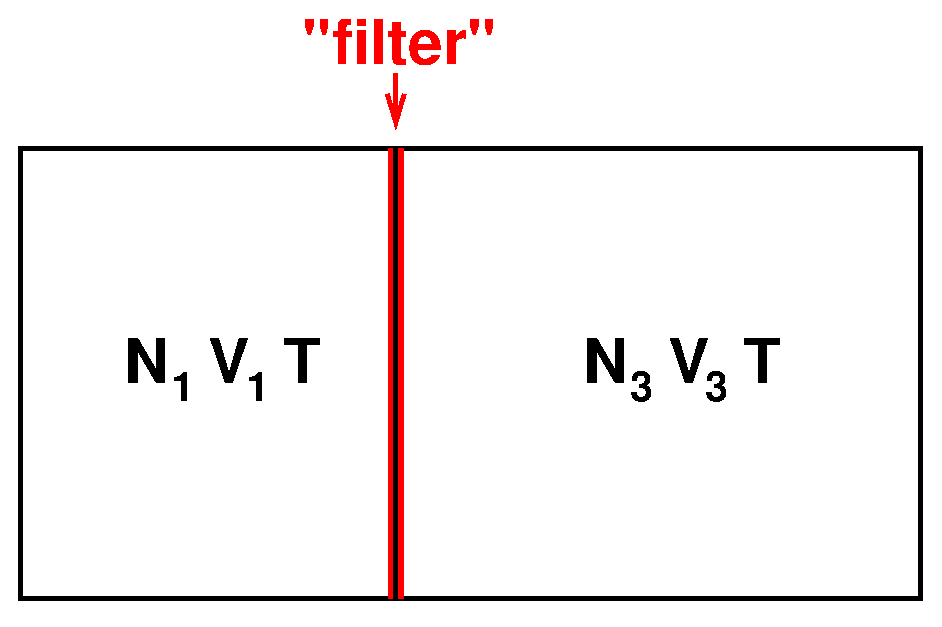
\includegraphics[width=0.6\textwidth]{fig.grand/partition.eps}    
  \end{minipage}
  % \begin{minipage}[t]{0.49\linewidth}
  % 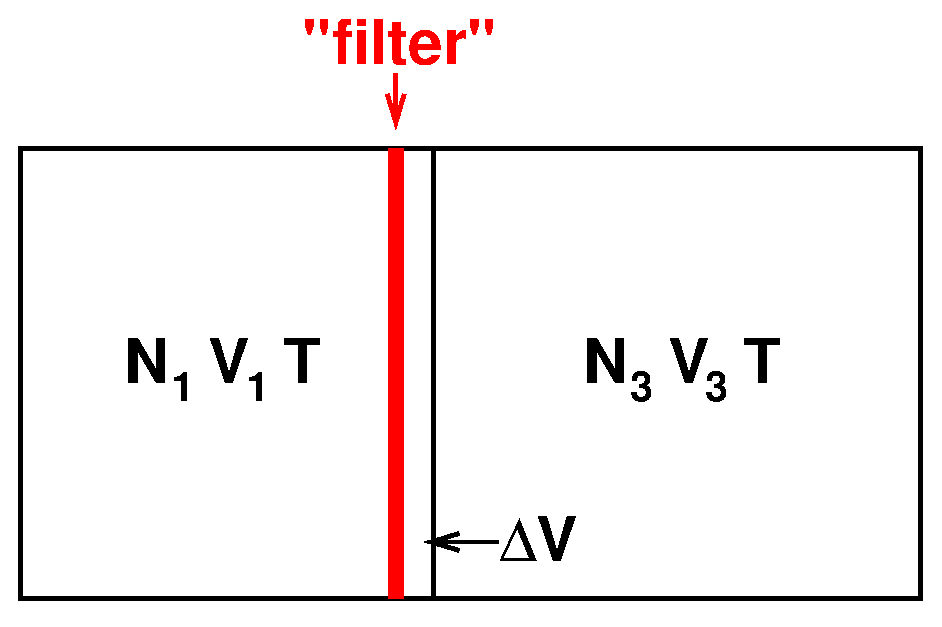
\includegraphics[width=0.6\textwidth]{fig.grand/partition-1.eps}    
  % \end{minipage}
  \caption{Schematic plot of the AdResS system in thermodynamic equilibrium. The thickness of the filter corresponds to $d_{\Delta}$.}
  \label{fig:tmp1}
\end{figure}
Here, two assumptions are made:
\begin{enumerate}\itemsep -1pt
\item $N_2\ {\ll}\ N_1 \ll N_3$: the second inequality corresponds to
  the thermodynamic limit of the Grand Canonical ensemble. The first
  one actually assumes that the $\HY$ region is infinitely thin so that it
  can be viewed as an infinitesimal membrane that allows free exchange of molecules from
  the AT region to the CG region and vice versa.
\item We now define a supplementary Hamiltonian:
  \begin{equation}
    \mathcal H(\vect x_1, N_1; \vect x_3, N_3) =
    \mathcal H_{N_1}^{\AT}(\vect x_1) + \mathcal H_{N_3}^{\CG}(\vect x_3); 
  \end{equation}
  The condition above is true, in the thermodynamic limit, if the system is
  short-range correlated.
\end{enumerate}
The equilibrium in the AT and CG region is assured by the membrane $\HY$ via the thermodynamic force. Conceptually, we assume there is an infinitely thin
``filter'' (see Fig.~\ref{fig:tmp1}) located at the interface between
the AT and CG regions. When a molecule travels from the CG region to
the AT region, the filter does some work $\omega_0$ on the system in order to assure the thermodynamic equilibrium between the AT and CG region.
Therefore, we add an empirical term in the Hamiltonian of the system
$N_1\omega_0$, related to the work done  by the filter. 
Having fixed the number of molecules in the three regions, and by following the
arguments of the last section, both the AT and the CG regions are
subject to the Boltzmann distribution.
Thus, the fixed-number partition function ($N_1$ in the AT region and $N_3$ in the CG region) of the system reads
\begin{align}\nonumber
  q(N,V,T)
  &= \frac1{N!}\int
  \dd d\vect x
  e^{-\beta
    [\mathcal H(\vect x_1, N_1; \vect x_3, N_3) +
    N_1\omega_0]}\\\nonumber
  &= \frac1{N!}\int
  \dd d\vect x_1\dd d\vect x_3\,
  e^{-\beta
    [\mathcal H_{N_1}^{\AT}(\vect x_1) +
    \mathcal H_{N_3}^{\CG}(\vect x_3) +
    N_1\omega_0]}\\\nonumber
  & = \frac{N_1!N_3!}{N!}
  e^{-\beta N_1\omega_0}
  \frac{1}{N_1!}\int\dd d\vect x_1 e^{-\beta\mathcal H_{N_1}^{\AT}(\vect x_1)}
  \frac{1}{N_3!}\int\dd d\vect x_3 e^{-\beta\mathcal H_{N_3}^{\CG}(\vect x_3)}\\
  & = \frac{N_1!N_3!}{N!}
  e^{-\beta N_1\omega_0}
  Q_{\AT}(N_1, V_1, T)\,
  Q_{\CG}(N_3, V_3, T) 
\end{align}
Considering the permutations of particles, the number of possibilities of
$N_1$ molecules being in the atomistic region and $N_3$ molecules being
in the coarse-grained region is  $\frac{N!}{N_1!N_3!}$.
Therefore, the partition function of the whole system reads
\begin{align}\nonumber
  Q(N,V,T) &= \sum_{N_1=1}^N
  \frac{N!}{N_1!N_3!} \frac{N_1!N_3!}{N!}
  e^{-\beta N_1\omega_0}
  Q_{\AT}(N_1, V_1, T)\,
  Q_{\CG}(N_3, V_3, T) \\
  &= \sum_{N_1=1}^N
  e^{-\beta N_1\omega_0}
  Q_{\AT}(N_1, V_1, T)\,
  Q_{\CG}(N_3, V_3, T) 
\end{align}
with natural relations:
\begin{align}
  N &= N_1 + N_3\\
  V &= V_1 + V_3
\end{align}
% The following approach can be found in, for example,
% Ref.~\cite{tuckeman2010statistical}.
First, for convenience, we denote that
\begin{align}
  \tilde q_{N_1} = 
  e^{-\beta N_1\omega_0}
  Q_{\AT}(N_1, V_1, T)\,
  Q_{\CG}(N - N_1, V_3, T),
\end{align}
and $\bar N_1$ is the value at which $\tilde q_{N_1}$ reaches
its maximum, namely $\tilde q_{\bar N_1} = \max \tilde q_{N_1}$.
Since $\tilde q_{N_1}$ is positive definite, a basic
observation is that
\begin{align}
  \tilde q_{\bar N_1}
  \leq
  \sum_{N_1=1}^N \tilde q_{N_1}
  \leq
  N \tilde q_{\bar N_1}. 
\end{align}
Due to the monotonicity of the logarithm, we have
\begin{align}
  \ln\tilde q_{\bar N_1}
  \leq
  \ln\sum_{N_1=1}^N \tilde q_{N_1}
  \leq
  \ln (N \tilde q_{\bar N_1})
  =
  \ln N + \ln\tilde q_{\bar N_1}.
\end{align}
If $\ln N \ll \ln \tilde q_{\bar N_1}$ (the validity will be discussed
later), then 
\begin{align}
  \ln\sum_{N_1=1}^N \tilde q_{N_1}
  \approx
  \ln\tilde q_{\bar N_1},
\end{align}
which is
\begin{align}
  \ln Q(N, V, T)
  \approx
  -\beta \bar N_1\omega_0 + 
  \ln Q_{\AT}(\bar N_1, V_1, T) + \ln Q_{\CG}(N - \bar N_1, V_3, T)
\end{align}
or equivalently
\begin{align}\label{eqn:a-energy-1}
  A(N, V, T)
  \approx
  \bar N_1\omega_0 +
  A_{\AT}(\bar N_1, V_1, T) + A_{\CG}(N - \bar N_1, V_3, T)
\end{align}
Where $A$ denotes the Helmholtz free energy. 
At this point, the crucial question is if the condition $\ln N \ll \ln \tilde q_{\bar N_1}$
holds, or equivalently
\begin{align}\label{eqn:condition}
  \ln N 
  \ll
  -\beta \bar N_1\omega_0 +
  \ln Q_{\AT}(\bar N_1, V_1, T) + \ln Q_{\CG}(N - \bar N_1, V_3, T)
\end{align}
Generally this is true: $\ln Q_{\CG}(N - \bar N_1, V_3, T)$
is proportional to the free energy $A_{\CG}(N - \bar N_1, V_3, T)$,
which is an extensive thermodynamic variable, so
$A_{\CG}(N - \bar N_1, V_3, T)$ is proportional to $N-\bar N_1$.
Due to the thermodynamic limit $N \gg \bar N_1$,
$A_{\CG}(N - \bar N_1, V_3, T)$ is actually proportional $N$, which
is much larger than $\ln N$ under thermodynamic limit; this
validates condition~\eqref{eqn:condition}.
We will see later (from Eqn.~\eqref{eqn:pn1})
that the maximum $\bar N_1$ corresponds to the maximum
value of probability $p(N_1)$; this is also the average molecule
number in the AT region that is of statistical importance
under the thermodynamic limit.  Since $\bar
N_1$ is the maximum, by differentiating on the right hand side of
Eqn.~\eqref{eqn:a-energy-1}, we have the relation:
\begin{align}
  \omega_0 = \mu_{\CG}(N - \bar N_1, V_3, T)  - \mu_{\AT}(\bar N_1, V_1, T)
\end{align}
This means that the difference in the chemical potential between the AT and CG
regions is taken care by the work of the filter.
Now, if the thermodynamic force of Eq.\ref{thf} ensures an
equilibrium that is the same as the full atomistic reference system,
the related work produced by the thermodynamic force is nothing else than $\omega_0 $.
In turn, this implies that the thermodynamic force assures the balance between the chemical potentials of the AT and CG resolution,
namely:
\begin{align}\label{eqn:w-mu-diff}
  \omega_0 = \mu_{\CG}(\rho_0V_3, V_3, T) - \mu_{AT}(\rho_0 V_1, V_1, T)
\end{align}
$\rho_0$ is the number density at which the atomistic and coarse-grained
resolutions should match,
namely $\bar N_1 = \rho_0V_1$ and $N - \bar N_1 = \rho_0(V - V_1)$ should apply.
Eqn.~\eqref{eqn:w-mu-diff} is a necessary
condition for the thermodynamic force that ensures
the correct equilibrium of the AT and CG regions.\\

\noindent
On the other hand, if we translate from the language of Helmholtz free
energy into that of the grand potential, we have that
under the thermodynamic limit, they are the same.
Next, assuming the system reaches an
equilibrium of flat density profile of $\rho_0$ all over the AdResS simulation box, 
Eqn.~\eqref{eqn:a-energy-1} becomes:
\begin{align}\label{eqn:g-energy-1}
  G(\mu, V, T) \approx
  \rho_0V_1\omega_0
  + G_{\AT}(\mu_{\AT}, V_1, T) + G_{\CG}(\mu_{\CG}, V - V_1, T)
\end{align}
where
\begin{align}
  G(\mu, V, T) = A(N, V, T) - \mu_{\AT} \bar N_1 - \mu_{\CG}(N - \bar N_1)
\end{align}
Because of the equilibrium situation, the derivative of r.h.s. of
Eqn.~\eqref{eqn:g-energy-1} with respect to atomistic volume $V_1$
should vanishes (the same argument as the Helmholtz free energy):
\begin{align}
  \rho_0\omega_0 = -p_{\AT}+p_{\CG} \quad\Longrightarrow\quad
  p_{\AT} + \rho_0\omega_0 = p_{\CG}
\end{align}
which is exactly the definition of the thermodynamic force.
The argument in this section is based on the fact that $\bar N_{1}$, rather than $N_{1}$ can be considered as representative of the configuration realizations in the AT region. This implies that the particle fluctuations, $\Delta N_{1}$,
are negligible (compared to $\bar N_{1}$) in the AT region. This hypothesis is valid if the AT region is large enough so that $\bar N_{1}$ is large. This point seems to be true in all numerical experiments done so far (see e.g. Ref.\cite{debash}). In this way, we have shown the formal derivation of the thermodynamic force as a tool to balance the chemical potential between the two regions. For a Grand Canonical-like set up, the balance of chemical potential between open regions is a necessary condition to have the exchange of molecules in thermodynamic equilibrium and as a consequence we have formally justified why Eq.\ref{thf} is a necessary condition for AdResS to be considered an effective Grand Canonical set up.

\subsection{The number probability $p(N_1)$}
In this section, we define at which level of approximation $p(N_{1})$, in AdResS is the same as in a full atomistic simulation. This must be done in order to justify the reliability of AdResS as a Grand Canonical set up in terms of probability distribution. In fact if  $p(N_{1})$ in AdResS is very different from the corresponding one of a full atomistic simulation, then clearly the AdResS method cannot be considered to provide realistic results since the artifacts due to the different $p(N_{1})$ would give a not realistic description of the system. 
Let us consider the marginal distribution $p(N_1)$
\begin{align}\nonumber
  p(N_1)
  &=
  \frac{N!}{N_1!N_3!}
  \int
  \dd d\vect x_1\dd d\vect x_3  \:
  \frac{1}{Q(N,V,T) N!}
  e^{-\beta
    [\mathcal H_{N_1}^{\AT}(\vect x_1) +
    \mathcal H_{N_3}^{\CG}(\vect x_3) +
    N_1\omega_0]}\\\nonumber
  &=
  \frac{N!}{N_1!N_3!}
  \frac{N_1!N_3!}{Q(N,V,T) N!}
  e^{-\beta N_1\omega_0}
  \bigg[
  \frac1{N_1!}
  \int
  \dd d\vect x_1
  e^{-\beta \mathcal H_{N_1}^{\AT}(\vect x_1)}
  \bigg]
  \bigg[
  \frac1{N_3!}
  \int
  \dd d\vect x_3
  e^{-\beta \mathcal H_{N_3}^{\CG}(\vect x_3)}
  \bigg]  \\\label{eqn:pn1}
  &=
  \frac
  {
    e^{-\beta N_1\omega_0}
    Q_{\AT}(N_1,V_1,T) Q_{\CG}(N-N_1,V_3,T)
  }
  {
    \sum_{n_1}
    e^{-\beta n_1\omega_0}
    Q_{\AT}(n_1,V_1,T) Q_{\CG}(N-n_1,V_3,T)
  }
\end{align}
where $n_1$ is the summation variable that goes from 0 to $N$.
In any case, when $n_1$ is not much smaller than $N$ (i.e. out of the range of the
thermodynamic limit), the statistic is not relevant,
and can be safely neglected.
The marginal number distribution of the full atomistic simulation,
which the AdResS simulation should
reproduce is
\begin{align}
  p_{\AT}(N_1)
  &=
  \frac
  {
    Q_{\AT}(N_1,V_1,T) Q_{\AT}(N-N_1,V_3,T)
  }
  {
    \sum_{n_1}
    Q_{\AT}(n_1,V_1,T) Q_{\AT}(N-n_1,V_3,T)
  }  
\end{align}
We want to calculate the difference between $p(N_1)$ and $p_{\AT}(N_1)$; that is the difference between the particle probability in the atomistic region of AdResS ($p(N_{1})$), and the particle probability in a full atomistic simulation in the region equivalent to the AT region of AdResS.
In order to do so we proceed with the following technical operation: multiply the numerator of $p(N_1)$ by the denominator of
$p_{\AT}(N_1)$ (denoted by $T_1$),
and multiply the numerator of $p_{\AT}(N_1)$
by the denominator of $p(N_1)$ (denoted by $T_2$). It follows:
\begin{align}
  T_1
  &=
  e^{-\beta N_1\omega_0}
  Q_{\AT}(N_1,V_1,T) Q_{\CG}(N-N_1,V_3,T)
  \times
  \sum_{n_1}
  Q_{\AT}(n_1,V_1,T) Q_{\AT}(N-n_1,V_3,T)\\
  T_2
  &=
  Q_{\AT}(N_1,V_1,T) Q_{\AT}(N-N_1,V_3,T)
  \times
  \sum_{n_1}
  e^{-\beta n_1\omega_0}
  Q_{\AT}(n_1,V_1,T) Q_{\CG}(N-n_1,V_3,T)
\end{align}
The difference between $T_1$ and $T_2$ is basically the difference
between $p(N_1)$ and $p_{\AT}(N_1)$.
Calculating $T_1$:
\begin{align}\nonumber
  T_1
  &=
  \sum_{n_1}
  e^{-\beta N_1\omega_0}
  Q_{\AT}(n_1,V_1,T)\,
  Q_{\AT}(N_1,V_1,T)\,
  Q_{\AT}(N-n_1,V_3,T)\,
  Q_{\CG}(N-N_1,V_3,T) \\\label{eqn:t1-1}
  &=
  \sum_{n_1}
  \exp
  \big\{-\beta
  \big[
  \omega_0N_1 +
  A_{\AT}(n_1,V_1,T) +
  A_{\AT}(N_1,V_1,T) +
  A_{\AT}(N-n_1,V_3,T) +
  A_{\CG}(N-N_1,V_3,T)
  \big]
  \big\}
\end{align}
Since we work under the hypothesis that the atomistic region is much smaller than the whole system, it
is reasonable to assume $n_1 \ll N$ and $N_1\ll N$.
Notice the free energy is extensive.
Due to the Euler's theorem~\cite{tuckeman2010statistical},
we have
\begin{align}\label{eqn:Aat-0}
  A_{\AT}(N-n_1,V_3,T)
  &= V_3 A_{\AT}(\frac{N-n_1}{V_3},1,T)
  = V_3 A_{\AT}(\rho_0 + \frac{\hat N_1 - n_1}{V_3},1,T)\\\label{eqn:Acg-0}
  A_{\CG}(N-N_1,V_3,T)
  &= V_3 A_{\CG}(\frac{N-N_1}{V_3},1,T)
  = V_3 A_{\CG}(\rho_0 + \frac{\hat N_1 - N_1}{V_3},1,T),
\end{align}
where $\hat N_1$ is the number of molecules in the atomistic region
at the wished density $\rho_0$ of equilibrium, namely
$\hat N_1 = \rho_0V_1 = N - \rho_0 V_3$.
Notice, under the thermodynamic limit, $\hat N_1$ is equivalent to
$\bar N_1$.
$A_{\AT}(\rho_0 + (\hat N_1 - n_1)/{V_3},1,T)$ and
$A_{\CG}(\rho_0 + (\hat N_1 - N_1)/{V_3},1,T)$ are
the free energies per \emph{unit} volume, with
the density perturbed from $\rho_0$ by  $(\hat N_1 - n_1)/{V_3}$
and $(\hat N_1 - N_1)/{V_3}$, respectively.
These perturbations originate from the fluctuating
number of molecules in the atomistic region: when the number
deviates from $\hat N_1$, molecules enter into the coarse-grained
region and the density is perturbed.
Under the thermodynamic
limit, $\hat N_1$ is comparable to $n_1$ and $N_1$, and all of them are
supposed to be much much smaller than $N$ while $V_3$ is of the same order of magnitude of $V$ (the large CG region compared to the small AT region).
Since $\rho_0 = N/V$ always holds, the perturbations
$(\hat N_1 - n_1)/{V_3}$
and $(\hat N_1 - N_1)/{V_3}$ are small.
Therefore, we have the following
Taylor expansions of the free energies \eqref{eqn:Aat-0} and \eqref{eqn:Acg-0}
about $\rho_0$:
\begin{align}
  A_{\AT}(\rho_0 + \frac{\hat N_1 - n_1}{V_3},1,T)
  &= A_{\AT}(\rho_0,1,T)
  +\mu_{\AT}
  \Big(
  \frac{\hat N_1 - n_1}{V_3}
  \Big)
  +
  \frac1{2\rho_0^2\,\kappa_{\AT}}
  \Big(
  \frac{\hat N_1 - n_1}{V_3}
  \Big)^2
  + \textrm{h.o.t.} \\
  A_{\CG}(\rho_0 + \frac{\hat N_1 - N_1}{V_3},1,T)
  &= A_{\CG}(\rho_0,1,T)
  +\mu_{\CG}
  \Big(
  \frac{\hat N_1 - N_1}{V_3}
  \Big)
  +
  \frac1{2\rho_0^2\,\kappa_{\CG}}
  \Big(
  \frac{\hat N_1 - N_1}{V_3}
  \Big)^2
  + \textrm{h.o.t.} 
\end{align}
The ``h.o.t.'' stands for higher order terms (greater than 2)
of the density perturbation, which we neglect since they have been found numerically not relevant (see Ref.\cite{rdfcorr}).
By using the conditions on the balance of the chemical potential derived in the previous section:
\begin{align}\label{eqn:mu-eq}
  \mu_{\CG} &= \mu_{\AT} + \omega_0\\\label{eqn:kappa-eq}
  \kappa_{\CG} &= \kappa_{\AT}
\end{align}
We have $T_1$
\begin{align}\nonumber
  T_1
  = \,&
  \sum_{n_1}
  \exp
  \Big\{-\beta
  \Big[
  A_{\AT}(n_1,V_1,T) +
  A_{\AT}(N_1,V_1,T) +
  A_{\AT}(\rho_0V_3,V_3,T) +
  A_{\CG}(\rho_0V_3,V_3,T) \\
  \,&+(\mu_\AT + \mu_\CG)\hat N_1
  -\mu_{\AT}\,(N_1 + n_1) +
  \frac{V_3}{2\rho_0\, \kappa_{\AT}}
  \Big[
  \Big(
  \frac{\hat N_1 - n_1}{V_3}
  \Big)^2
  +
  \Big(
  \frac{\hat N_1 - N_1}{V_3}
  \Big)^2
  \Big]
  +\textrm{h.o.t.}
  \Big]
  \Big\}
\end{align}
Similarly, we calculate $T_2$:
\begin{align}\nonumber
  T_2
  &=
  \sum_{n_1}
  e^{-\beta n_1\omega_0}
  Q_{\AT}(n_1,V_1,T)\,
  Q_{\AT}(N_1,V_1,T)\,
  Q_{\CG}(N-n_1,V_3,T)\,
  Q_{\AT}(N-N_1,V_3,T) \\\nonumber
  &=
  \sum_{n_1}
  \exp
  \big\{-\beta
  \big[
  \omega_0n_1 +
  A_{\AT}(n_1,V_1,T) +
  A_{\AT}(N_1,V_1,T) +
  A_{\CG}(N-n_1,V_3,T) +
  A_{\AT}(N-N_1,V_3,T)
  \big]
  \big\}
\end{align}
with similar expansions and by the conditions Eqn.~\eqref{eqn:mu-eq}
and \eqref{eqn:kappa-eq}, we have:
\begin{align}\nonumber
  T_2
  = \,&
  \sum_{n_1}
  \exp
  \Big\{-\beta
  \Big[
  A_{\AT}(n_1,V_1,T) +
  A_{\AT}(N_1,V_1,T) +
  A_{\AT}(\rho_0V_3,V_3,T) +
  A_{\CG}(\rho_0V_3,V_3,T) \\
  \,&+(\mu_\AT + \mu_\CG)\hat N_1
  -\mu_{\AT}\,(N_1 + n_1) +
  \frac{V_3}{2\rho_0\, \kappa_{\AT}}
  \Big[
  \Big(
  \frac{\hat N_1 - n_1}{V_3}
  \Big)^2
  +
  \Big(
  \frac{\hat N_1 - N_1}{V_3}
  \Big)^2
  \Big]
  +\textrm{h.o.t.}
  \Big]
  \Big\}
\end{align}
Comparing $T_1$ and $T_2$, one can easily see that they are equivalent (at least) to the second leading
order with respect to the density perturbations
$(\hat N_1 - n_1)/{V_3}$
and $(\hat N_1 - N_1)/{V_3}$.
Since the difference between the probabilities
$p(N_1)$ and $p_{\AT}(N_1)$ is basically the difference between $T_1$
and $T_2$, we conclude that $p(N_1)$ is a good approximation to
$p_{\AT}(N_1)$ to the second leading order. High orders, as anticipated before, seem numerically not relevant and anyway, at this stage, not easy to treat at formal level.


\section{A numerical test}
\begin{figure}
  \centering
  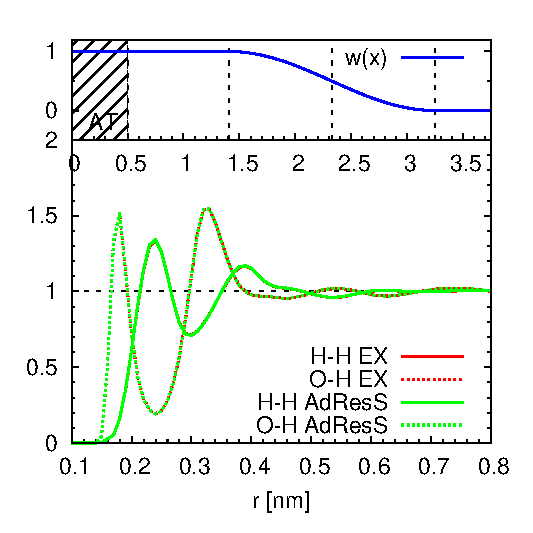
\includegraphics[width=0.245\textwidth]{fig.grand/rdf-hhoh-375-425.eps}
  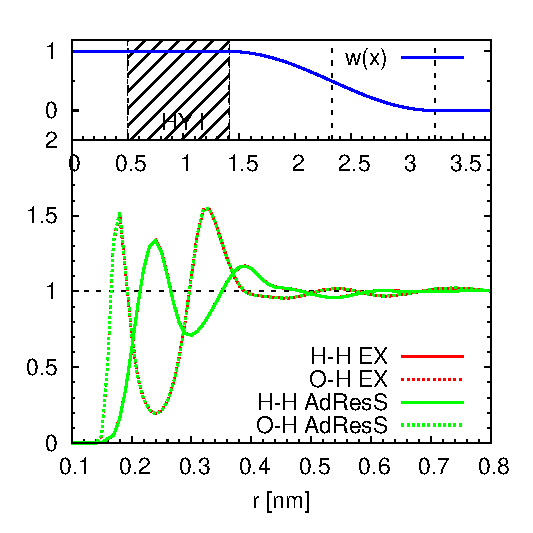
\includegraphics[width=0.245\textwidth]{fig.grand/rdf-hhoh-425-516.eps}
  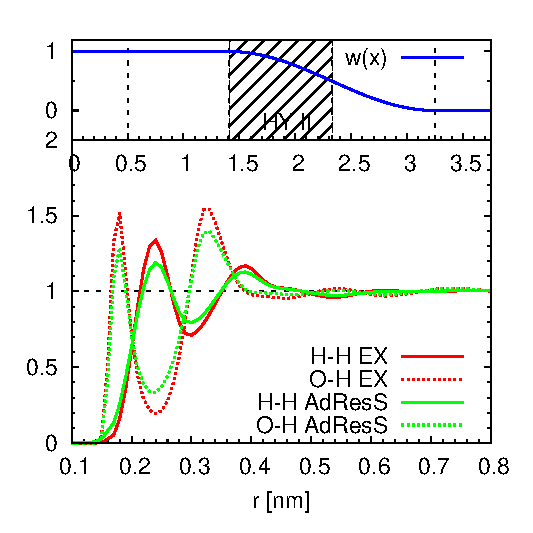
\includegraphics[width=0.245\textwidth]{fig.grand/rdf-hhoh-516-608.eps}
  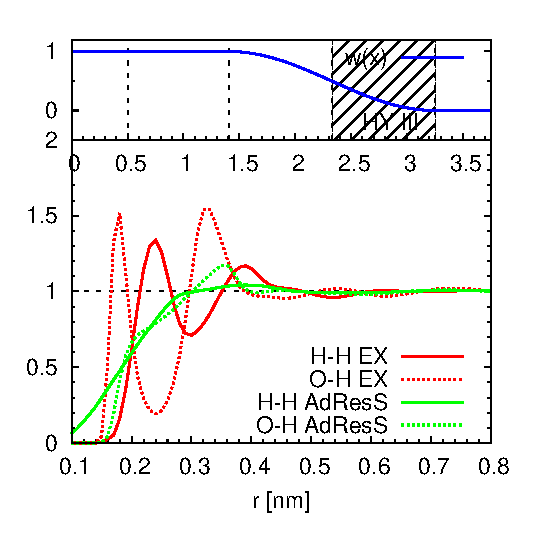
\includegraphics[width=0.245\textwidth]{fig.grand/rdf-hhoh-608-700.eps}
  \caption{Local H-H and O-H $g(r)$'s.
    The red line is the curve corresponding to the reference explicit (all atom)
    simulation (AT).
    The curve obtained by employing the AdResS 
    method is represented in green.
    The hybrid region is equally
    divided into three parts: HY I, HY II and HY III, the widths of
    which are roughly equal to the cut-off radius, i.e. 9 \textsf{nm}.    
    The top part of each panel shows the region where the $g(r)$ is calculated,
    and the value of weighting function $w(x)$ there.
    From left to right, the panels correspond to the AT region, 
    the HY I subregion of $\Delta$,
    the HY II subregion of $\Delta$,
    and the HY III subregion of $\Delta$, respectively. \recheck{It can be seen that beyond 0.5 \textsf{nm} the functions go to one, that is particle beyond this distance are uncorrelated; this is fully consistent with our hypothesis of Eq.\ref{eqn:p-1-2}.}}
  \label{fig:tmp2a}
\end{figure}

\begin{figure}
  \centering
  \includegraphics[width=0.9\textwidth]{fig.grand/fig-rdf3.more.eps}
  \caption{The 3-body correlation function.  The 1st row:
    atomistic.
    The 2nd to 5th row:
    AdResS with TIF-IBI correction in the AT, HY I, HY II, and HY III
    regions, respectively.
    Different columns give different distant between
    the first two molecules: from left to right $r_{12} =
    0.27\,\textsf{nm},\ 0.33\,\textsf{nm},\  
    0.80\,\textsf{nm}$.  The $x$ axis is the variable $h_1$, while $y$
    axis is the variable $h_2$ (please refer to the Appendix for the
    definition of these variables).  The magnitude that indicated by
    different colors presents the magnitude of $g^{(3)}$.
  }
  \label{fig:tmp2b}
\end{figure}

\recheck{The arguments we have used so far are not sufficient to infer that the probability $p(\vect x_1 , N_1)$, as presented in the theoretical anlysis, corresponds to that of a grand canonical distribution  Eqn.~\eqref{eqn:p}.
One must be very careful about any statement on $p(\vect x_1, N_1)$ 
due to the following three reasons:\\ 
1, The Boltzmann form of the distribution $p(\vect x_1|N_1; \vect x_2, N_2)$
is in this case only an approximation.\\
2, Conditions \eqref{eqn:p-1-cond1} and \eqref{eqn:p-1-cond2}
are only necessary, and are in general not sufficient to guarantee
the correct distribution $p(\vect x_2, N_2 | N_1)$ in the hybrid region $\HY$.\\ 3, The particle number distribution $p(N_1)$ is correct only up to the second order.\\
However, the number distribution $p(N_1)$ has already
been proved to be correct in Ref.~\cite{prlgc, rdfcorr} for the relevant case of liquid water and thus in this section, we want to test, with a numerical simulation, to what extent the configurational} {\bf WHAT EXACTLY MEANS CONFIGURATIONAL?   PLEASE SPECIFY}
\recheck{distribution is correct. 
Obviously it is a prohibitive task for any complex molecular system to determine the high-dimensional configurational distribution,
so, instead, we study its marginal distribution up to the third order.
Here we report the H-O and H-H RDFs (see Fig.~\ref{fig:tmp2a}), and the 3-body COM
RDF $g^{(3)}(\vect r_1, \vect r_2, \vect r_2)$ (see Fig.~\ref{fig:tmp2b}). For simulation
protocols and the definition of 3-body RDF, see the Appendix.
The first order marginal distribution, that is the molecular density profile and the second order marginal distribution, that is the COM RDF are not presented here, we address the readers to Ref.~\cite{rdfcorr}. 
Here we focus on the more delicate RDFs which involve the atomistic accuracy, and on the third order COM three-body distribution. From Fig.~\ref{fig:tmp2a} one can see that
the AdResS H-O and H-H RDFs are identical to those of 
the full atomistic reference system in the AT region.
Interestingly, despite the corrective force of the RFD is applied only to the COM RDF, also in the region HY I (that is close to the atomistic region) the H-O and H-H RDFs are the same as in the full atomistic case.
This implies that the AT region
is embedded in an environment where not only the COM but also finer structural
properties are the same as for the atomistic resolution.
In the HY II and III regions, the AdResS obviously deviate from the
full atomistic reference, because the atomistic nature 
is decreasing as a molecule travels from HY I to HY III, so it must be expected 
that the orientational order is also fading away. In HY III, the H-O and H-H
RDFs are actually structureless.
Furthermore, we test the 3-body COM RDF in Fig.~\ref{fig:tmp2b} (for the definition of the three-body COM RDF see Appendix~\ref{app:tmp1}).
Interestingly, the three -body correlation is correctly reproduced
by the AdResS in the AT and HY I  regions. This is a further strong argument in favor of the fact that in AdResS the AT region is embedded in a environment that, at least up to the three -body COM correlation is the same as the full atomistic reference system.
In the HY II and HY III regions, the three-body correlation deviates from the
full atomistic reference, when the first two molecules are near (the first
two columns). This means that reproducing only two-body COM RDF \emph{does not}
lead to the correct reproduction of the three-body COM RDF.
Another important information of Fig.~\ref{fig:tmp2a} and \ref{fig:tmp2b},
is that the hypothesis of short-range influence of a region over another employed in Eq.\ref{eqn:p-1-2} is numerically justified and thus we can state that for the case of liquid water at ambient conditions the AT region is only short-range
correlated with the rest of the system.} 


\section{Conclusions}
We have shown a detailed theoretical analysis about the validity, \recheck{the limitations} and meaning of the AdResS method within the framework of a Grand Canonical ensemble. Using strict formal arguments, we have interpreted the thermodynamic force, originally derived in an empirical way, as a tool to balance the difference in chemical potential due to the different resolutions in space. Finally, we have shown that, \recheck{under given hypothesis}, $p(N_{1})$, the probability distribution in the atomistic region of AdResS is equivalent to that in the same region in a full atomistic simulation, up to a second order expansion in the particle number density. \recheck{We have further strengthen our hypothesis and conclusions by carrying out a numerical experiment for the case of liquid water at ambient conditions where we could even go beyond the second order}. In conclusion, these results provide a solid theoretical basis to explain the numerical reliability of the AdResS as an effective Grand Canonical set up and provide basis for further formal and numerical development of the adaptive idea in terms of matching probability distributions.


\section*{Acknowledgement}
This work was partially supported by the Deutsche Forschungsgemeinschaft (DFG) with the Heisenberg grant provided to L.D.S (grant code DE 1140/5-1) and by ITN Nanopoly provided to H.W and C.S.
It was also supported in part by the National Science Foundation under Grant No. NSF PHY11-25915.



\section*{References}
\bibliography{ref}{}
\bibliographystyle{unsrt}


\appendix
\section{Simulation protocols}
The testing system contained 3456 SPC/E \cite{berendsen1987missing}
water molecules in a $7.50\textsf{nm}\times 3.72\textsf{nm}\times
3.72\textsf{nm}$ periodic box. The system was divided along the $x$ direction
into one atomistic region of width $1.00\textsf{nm}$ and one
coarse-grained region of width $1.00\textsf{nm}$ connected by two
hybrid region of width $2.75\textsf{nm}$.
The hybrid region was equally divided into three sub-regions (with width $\sim 0.9\textsf{nm}$)
to calculate the local RDFs.
These sub-regions are called HY I, HY II and HY III, from the AT side to the CG resolution side.
The simulation was made at
room temperature of $300\textsf{K}$. The time step was $\Delta t =
0.002\textsf{ps}$. The cut-off radius $r_{c}$ used for all interactions was
$0.90\textsf{nm}$. The electrostatic interaction method used for the
atomistic region was the reaction field method. All simulations were
performed by MD simulation software Gromacs \cite{gromacs}
and VOTCA \cite{ruehle2009versatile}.

\section{The details of the 3-body radial distribution function}
\label{app:tmp1}

\begin{figure}
  \centering
  \includegraphics[width=0.3\textwidth]{fig.grand/3mol.eps}
  \caption{The schematic plot of the 3-body RDF.}\label{fig:tmp3}
\end{figure}



The 3-body RDF is defined by
\begin{align}
  g^{(3)}(\vect r_1, \vect r_2, \vect r_3) =
  \frac{1}{\rho^3}N(N-1)(N-2) \,p^{(3)}(\vect r_1, \vect r_2, \vect r_3) 
\end{align}
where $p^{(3)}(\vect r_1, \vect r_2, \vect r_3) $ is the 3-body
probability distribution function. To plot this high-dimensional
distribution, we first fix the distance between molecule 1 and 2 (Mol
1 and 2 in Fig.~\ref{fig:tmp3}), then plot the RDF $g^{(3)}$ with
respect to the position of the third molecule (Mol 3 in
Fig.~\ref{fig:tmp3}).  The position of Mol 3 can be described by
the variables $h_1$ and $h_2$ in Fig.~\ref{fig:tmp3}, which are
the projection of Mol~3's position on the to the
axis defined by Mol 1 and 2, see Fig.~\ref{fig:tmp3}.




\end{document}